\documentclass[../homework.tex]{subfiles}

\pagestyle{fancy}
\fancyhf{}
\rhead{Hanzhi Zhou}
\lhead{Physics 2415 Homework}
\cfoot{\thepage}

\begin{document}
\subsection{Problem 8.2}
\subsubsection*{a)}
\begin{equation*}
	|\vec{E}| = \sqrt{E_0^2 \sin^2 (kz - \omega t) + E_0^2 \cos^2 (kz - \omega t)} = E_0
\end{equation*}

\subsubsection*{b)}
\begin{equation*}
	|\vec{B}| = \sqrt{B_0^2 \cos^2 (kz - \omega t) + B_0^2 \sin^2 (kz - \omega t)} = E_0
\end{equation*}

\subsubsection*{c)}
\begin{equation*}
	u = \frac{\epsilon_0}{2} E^2 + \frac{1}{2 \mu_0} B^2 = \epsilon_0 E^2
\end{equation*}

\subsubsection*{d)}
\begin{align*}
	\vec{E} \cdot \vec{B} & =
	\begin{bmatrix}
		E_0 \sin (kz - \omega t) \\
		E_0 \cos (kz - \omega t) \\
		0
	\end{bmatrix} \cdot
	\begin{bmatrix}
		-B_0 \cos (kz - \omega t) \\
		B_0 \sin (kz - \omega t)  \\
		0
	\end{bmatrix}   \\
	                      & = 0
\end{align*}

\subsubsection*{e)}
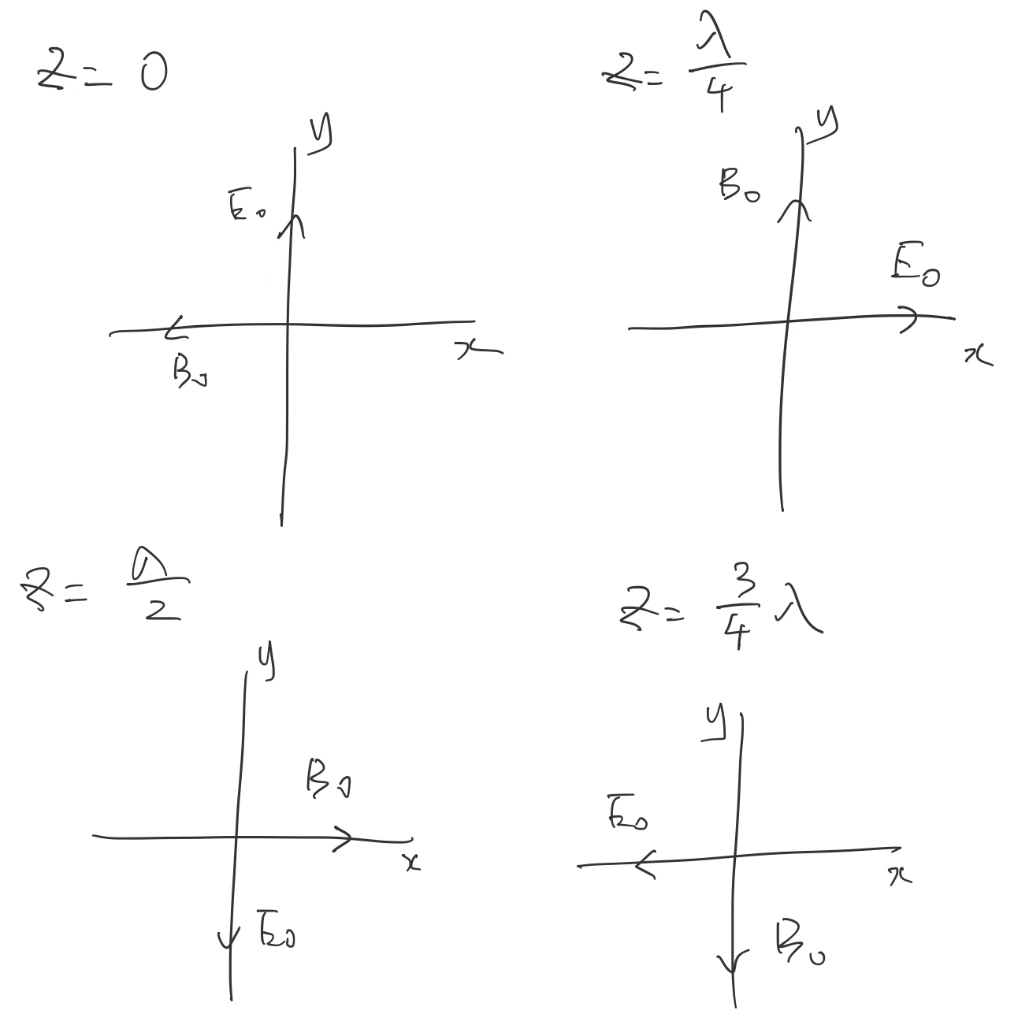
\includegraphics[width=.65\columnwidth]{p2-e.jpg}

\subsubsection*{f)}
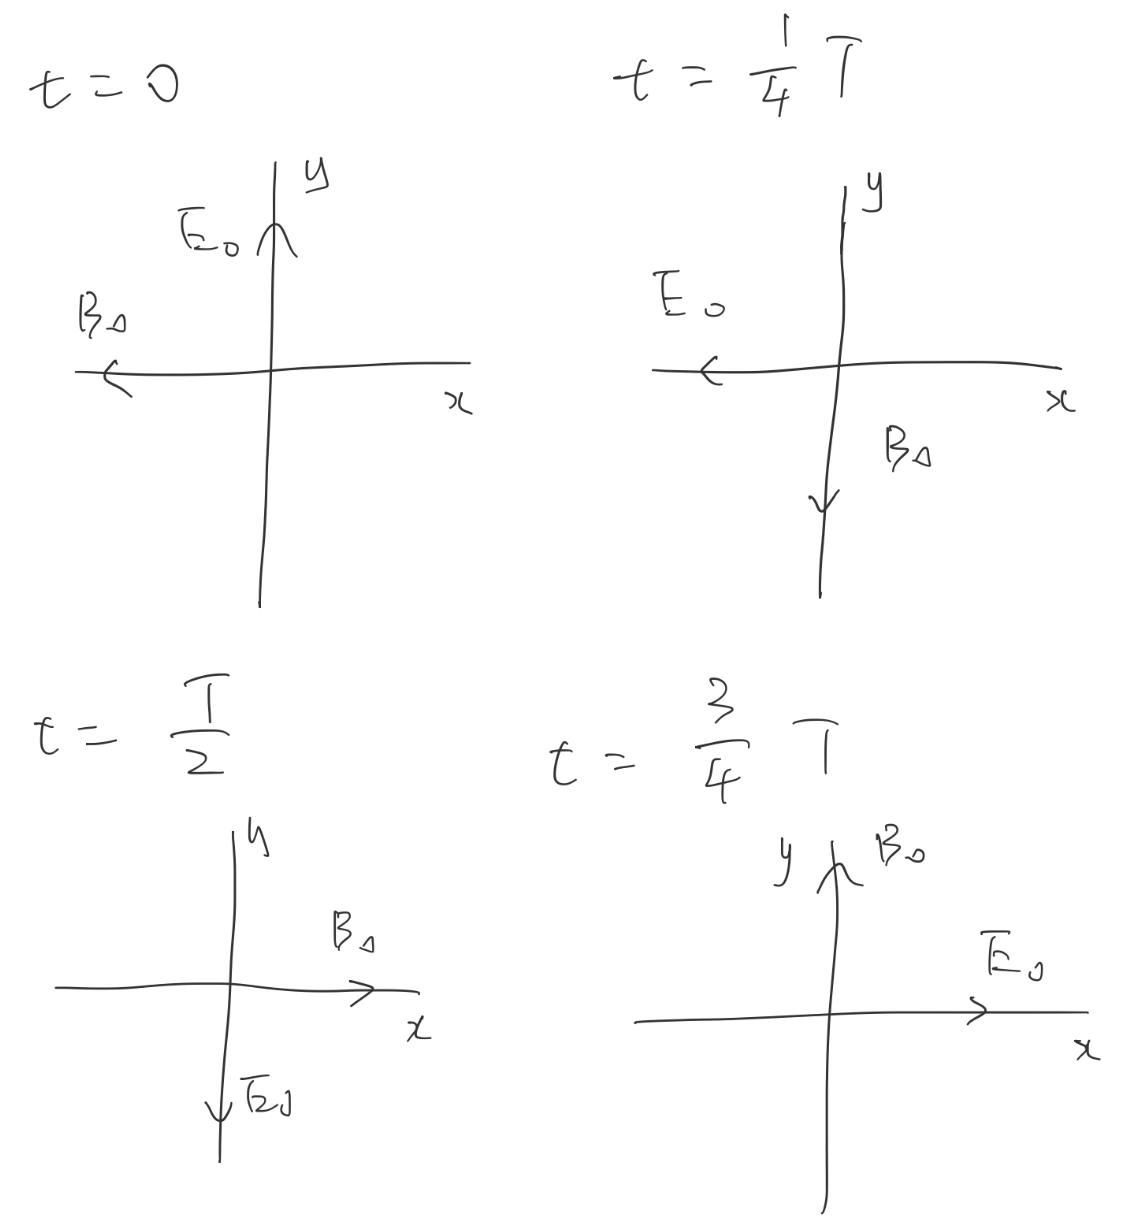
\includegraphics[width=.65\columnwidth]{p2-f.jpg}

\subsubsection*{h)}
\begin{align*}
	\vec{E} \times \vec{B} & =
	\begin{bmatrix}
		E_0 \sin (kz - \omega t) \\
		E_0 \cos (kz - \omega t) \\
		0
	\end{bmatrix} \times
	\begin{bmatrix}
		-B_0 \cos (kz - \omega t) \\
		B_0 \sin (kz - \omega t)  \\
		0
	\end{bmatrix}                                                                               \\
	                       & = E_0 B_0 \left(\sin^2 (kz - \omega t) + \cos^2 (kz - \omega t)\right) \hat{k} \\
	                       & = E_0 B_0 \hat{k}
\end{align*}

\subsubsection*{i)}
\begin{align*}
	f_1       & =
	\begin{bmatrix}
		E_0 \sin (kz - \omega t) \\
		0                        \\
		0
	\end{bmatrix} \times
	\begin{bmatrix}
		0                        \\
		B_0 \sin (kz - \omega t) \\
		0
	\end{bmatrix}                                                                  \\
	          & = E_0 B_0 \sin^2 (kz - \omega t) \hat{k}                                       \\
	f_2       & =
	\begin{bmatrix}
		0                        \\
		E_0 \cos (kz - \omega t) \\
		0
	\end{bmatrix} \times
	\begin{bmatrix}
		-B_0 \cos (kz - \omega t) \\
		0                         \\
		0
	\end{bmatrix}                                                                 \\
	          & = E_0 B_0 \cos^2 (kz - \omega t) \hat{k}                                       \\
	f_1 + f_2 & = E_0 B_0 \left(\sin^2 (kz - \omega t) + \cos^2 (kz - \omega t)\right) \hat{k} \\
	          & = E_0 B_0 \hat{k}
\end{align*}

\subsubsection*{j)}
Wave 1 oscillates in the $x$ direction. Wave 2 oscillates in the $y$ direction.
\end{document}